\documentclass[11pt]{article}
\usepackage[margin=0.8in]{geometry}
\usepackage{graphicx} % Required for inserting images
\setlength{\parindent}{0pt}
\usepackage{float}
\usepackage{caption}

\title{{\fontsize{21pt}{18pt}\selectfont COP290 Assignment - 1 Subtask - 3} \\ Trading Simulator and Analyzer}
\author{Yash Bansal \\ 2022CS51133 \and Shivam Sawarn \\ 2022CS11075}
\date{}
\begin{document}

\maketitle

\section{Introduction}

\begin{itemize}
    \item In this project, we have implemented different trading strategies, which, based on historical data, guide the user to buy or sell the stock.
    \item The strategies implemented are momentum-based strategies like Basic, n-day moving average (DMA) and stop-loss DMA (DMA++), and indicator analysis like MACD, RSI and ADX. A linear regression-based model is also used to predict the price.
    \item To get the best output, all the strategies are run in parallel, and the best profit and loss-giving strategy is finally chosen.
    \item Finally, trading strategies are implemented for co-related pairs of stocks, named mean-reverting pair trading strategy and stop-loss pair trading strategy.
\end{itemize}

\section{Implementation and Insights}
We implemented the following trading strategies and got many interesting insights into different algorithms and the parameters affecting them. We have plotted the graphs for Cash flow by applying the strategy for 15 years on SBIN stock and keeping the maximum number of stocks to 5, and we derived many interesting insights, as discussed below:- 

\subsection{Basic Strategy:-}
\begin{itemize}
    \item This is one of the most basic strategies:- If the price is increasing monotonically for the past n days, we buy a stock, hoping the price will increase.
    \item If the price is decreasing monotonically for the past n days, then we sell a stock, as the price may decrease more. So, we sell the stock to prevent loss.
    \item This is not a very good strategy, as the market changes very frequently, so to compare on the basis of just an increase or decrease in price will not give good results. It ignores the amount by which the market might have increased or decreased. Consequently, on applying the strategy for the last 15 years, very high loss of $>$ 13,000 is faced. This was the case when we could short-sell the stock.
    \item If we could not short-sell the stock, a slight less loss is faced and the final pnl came out to be -9,000.
    \item In this strategy we sell or buy only when the price changes are monotonic for n consecutive days so if there is a case when on one day there is positive increase and on its previous day we have decline in prices so we don't want them in our n days so we skip n days from that day as to getter better optimization in time complexity.
\end{itemize}

\begin{figure}[H]
  \centering
  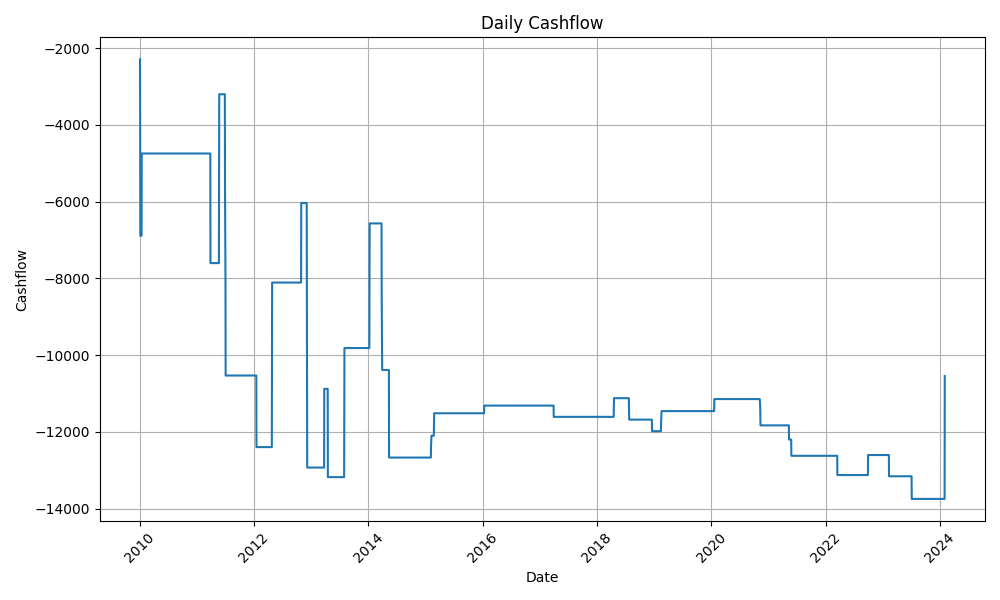
\includegraphics[width=1\textwidth]{Basic_with_short.png}
  \caption{Basic strategy Cashflow graph with short selling}
\end{figure}

\begin{figure}[H]
  \centering
  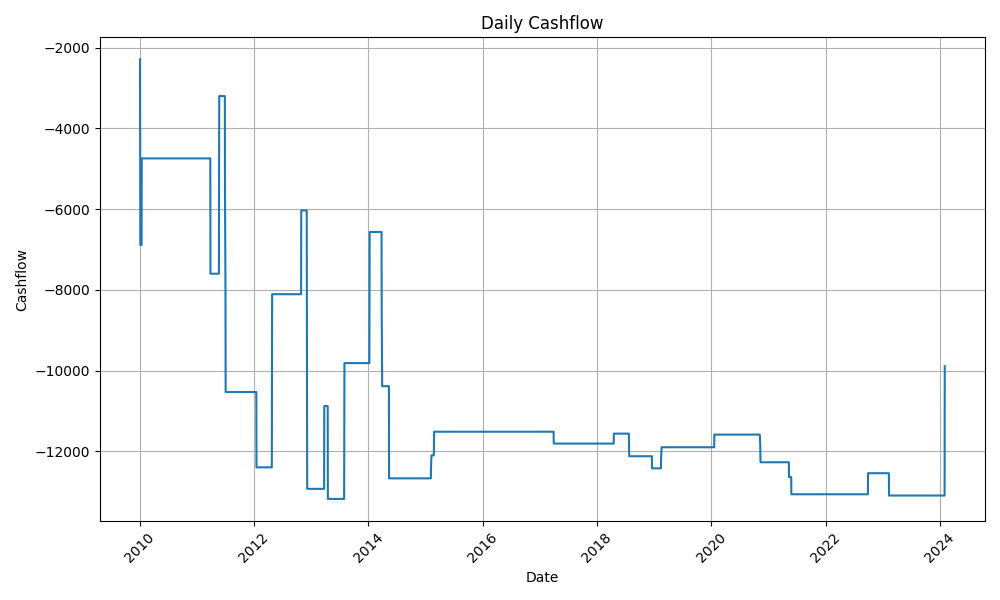
\includegraphics[width=1\textwidth]{Basic_without_short.png}
  \caption{Basic strategy Cashflow graph without short selling}
\end{figure}

\subsection{n - Day Moving Average (DMA):-}
\begin{itemize}
    \item In this strategy, we first calculate the average of the last n days' prices and also their standard deviation. If the current price > mean + p time standard deviation, where p is a constant, then we buy the stocks.
    \item If the current price is less than the mean - p times standard deviation, then we sell the stock, as this indicate that the stock price is going down, which indicates to sell the stock.
    \item Here, we need to carefully consider the values of n and p, as slight changes in these parameters can affect the algorithm significantly.
    \item But this kind of strategy is not good for highly fluctuating markets, as these can have a very high standard deviation, which could hen generate wrong signals, leading to high losses.
    \item On applying this strategy on the data considered above, this strategy still gave a high loss, comparatively less loss than the basic strategy. On assuming short selling, it gave a loss of about 11,000.
    \item On the other hand, while assuming no short selling, the strategy gave a loss of 10,000. Thus, in this strategy also, short selling does not perform better than no short selling startegy.
\end{itemize}

\begin{figure}[H]
  \centering
  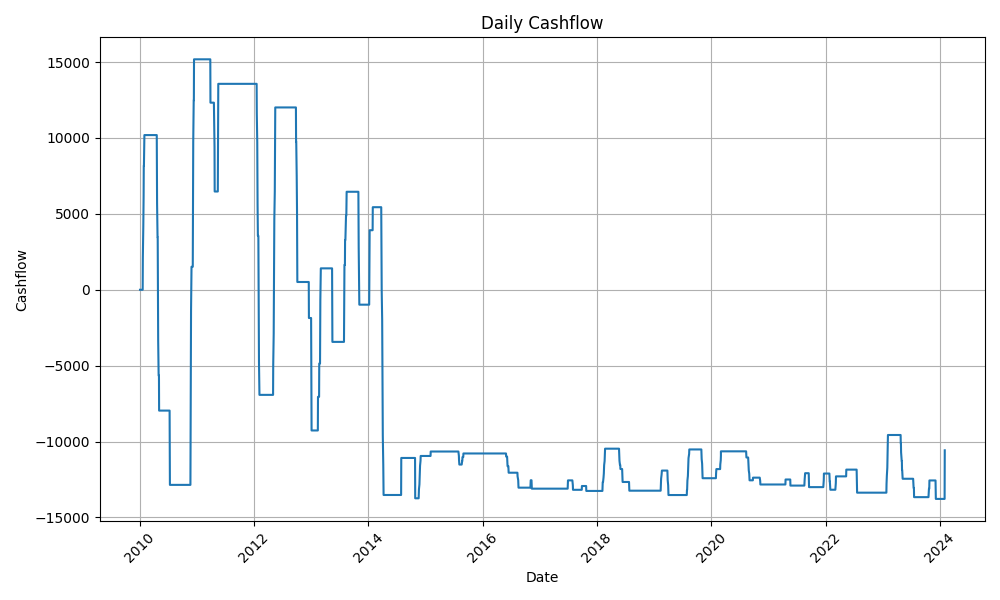
\includegraphics[width=1\textwidth]{DMA_with_short.png}
  \caption{DMA strategy Cashflow graph with short selling}
\end{figure}

\begin{figure}[H]
  \centering
  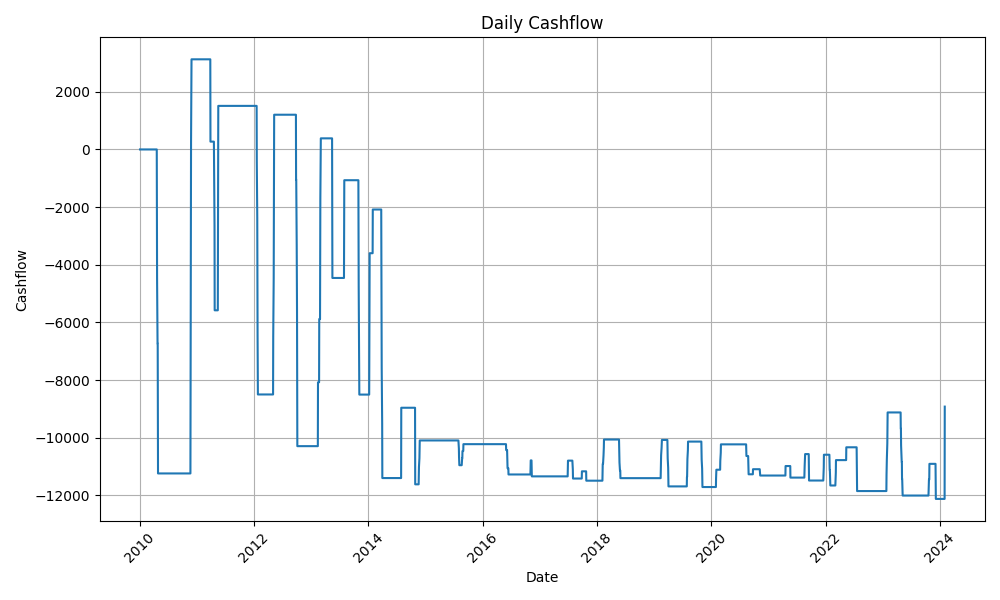
\includegraphics[width=1\textwidth]{DMA_without_short.png}
  \caption{DMA strategy Cashflow graph without short selling}
\end{figure}

\subsection{Stop - Loss DMA (DMA++):-}
\begin{itemize}
    \item This strategy is similar to DMA, but with two features incorporated into the older algorithm:- Stop - loss method and smoothing factor.
    \item In stop-loss method, if a particular stock is held for more than max\_hold\_days, then we forcefully sell the stock, so as to avoid losing more money. For the smoothing factor, we calculate the adaptive moving average and efficiency ratio.
    \item This strategy has two main parameters:- c1 and c2, and their values can highly affect out algorithm. So choosing good c1 and c2 is very important. We took c1 = 2 and c2 = 0.2.
\end{itemize}

\subsection{Moving Average Convergence Divergence (MACD):-}
\begin{itemize}
    \item It calculates the difference between two exponential moving averages (EMA) of price data (one short-term and one long-term), then generates a signal line based on another EMA of the MACD itself. Buying or selling signals are generated based on the relationship between the MACD and its signal line.
    \item It give more weight to the recent prices, thus gives better results on real data. But it is not very compatible with sudden market fluctuations.
    \item With assuming short selling, it gave a very less loss of just about 1200. Thus, it is very much better compared to the previously discussed algorithms. But while assuming no short selling, it gave a high loss of about 8000.
    \item Thus, short selling is very useful while trading through MACD algorithm.
\end{itemize}

\begin{figure}[H]
  \centering
  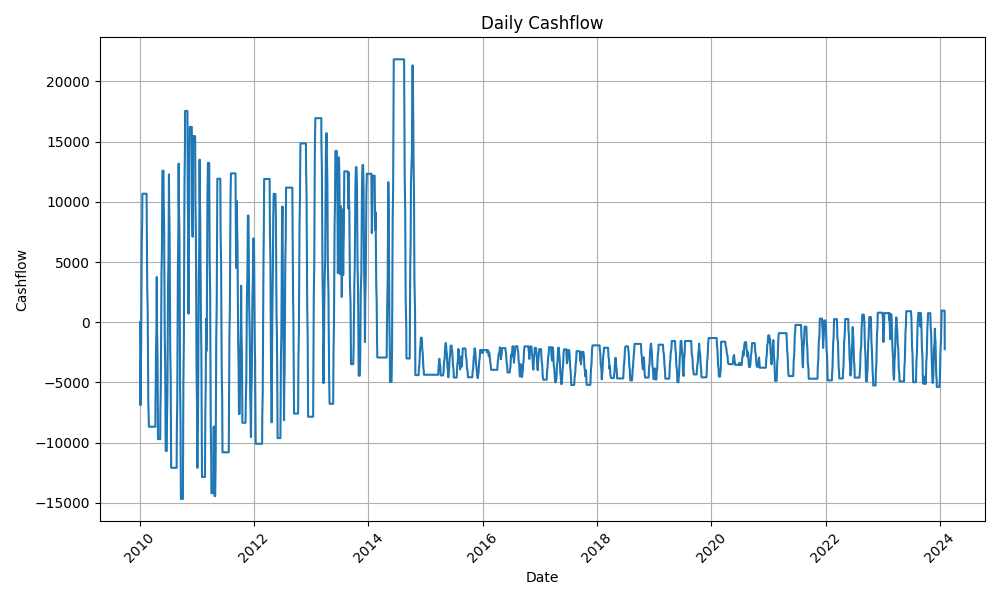
\includegraphics[width=1\textwidth]{MACD_with_short.png}
  \caption{MACD strategy Cashflow graph with short selling}
\end{figure}

\begin{figure}[H]
  \centering
  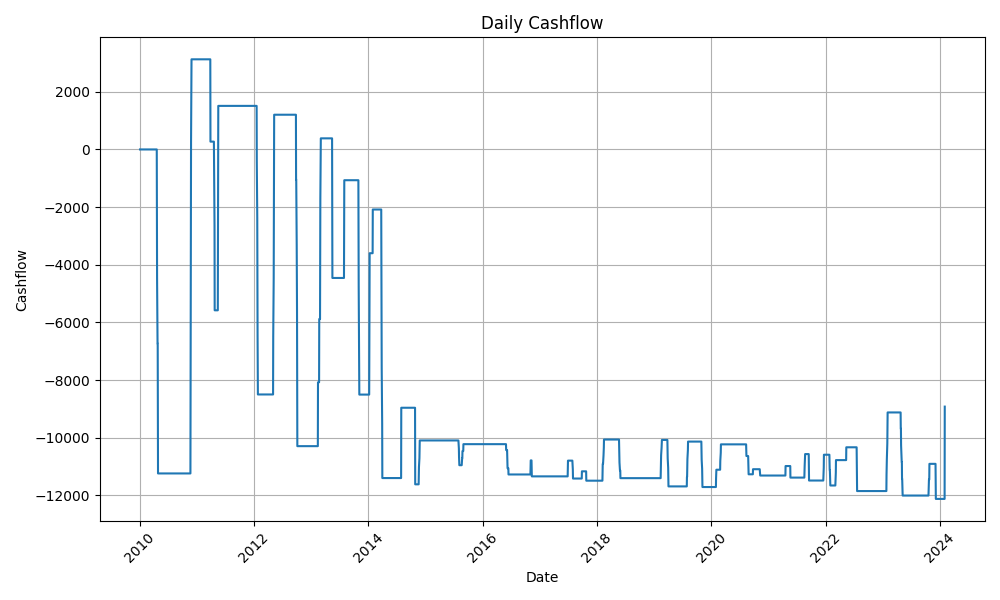
\includegraphics[width=1\textwidth]{DMA_without_short.png}
  \caption{MACD strategy Cashflow graph without short selling}
\end{figure}

\subsection{Relative Strength Index (RSI):-}
\begin{itemize}
    \item It calculates the relative strength of gains versus losses over a specified period to determine the market's potential overbought or oversold conditions. When the RSI crosses an oversold threshold, a buy signal is generated, and a sell signal is triggered when it crosses above an overbought threshold.
    \item It is highly customizable over different trading styles and timeframes.
    \item But similar to MACD, it also lags behind sudden price movements.
    \item When applied to the real data, It gave a very high profit of about 9,000 when short selling is assumed.
    \item But when short selling is not considered, the algorithm gave a loss of about 1,000. Thus in this algorithm also, short selling performs much better than no short selling.
\end{itemize}

\begin{figure}[H]
  \centering
  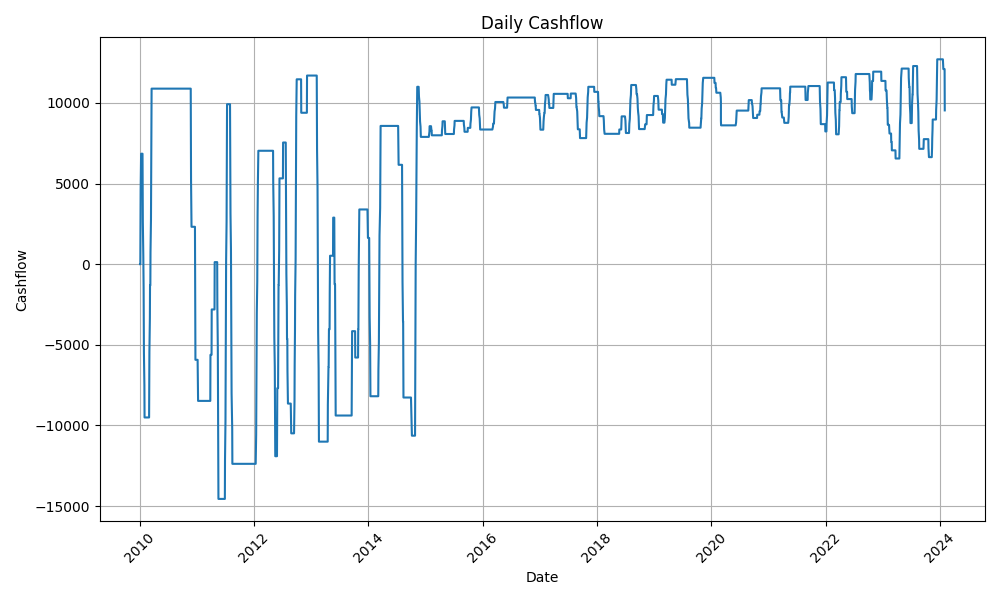
\includegraphics[width=1\textwidth]{RSI_with_short.png}
  \caption{RSI strategy Cashflow graph with short selling}
\end{figure}

\begin{figure}[H]
  \centering
  \includegraphics[width=1\textwidth]{RSi_without_short.png}
  \caption{RSI strategy Cashflow graph without short selling}
\end{figure}

\subsection{Average Directional Index (ADX):-}
\begin{itemize}
    \item It calculates the strength of a trend by measuring the average movement of price over a specified period. It involves several steps, including calculating the True Range (TR), Directional Movement (DM), Average True Range (ATR), Directional Indexes (DI), and ultimately the ADX itself.
    \item A buy signal is generated if the ADX exceeds a specified threshold, while a sell signal is triggered if the ADX falls below the threshold.
    \item This algorithm is less sensitive to market flunctuations, thus is suitable for trend following strategies. Also, it can be easily integrated with other algorithms to give much better results.
    \item This algorithm alone cannot give good statistics about the market, and need to be integrated with other strategies, otherwise it may lead to inefficient trades.
    \item it gave a very high profit of about 7000 when we assumed short selling, and almost no profit or loss when short selling is not assumed.
\end{itemize}

\begin{figure}[H]
  \centering
  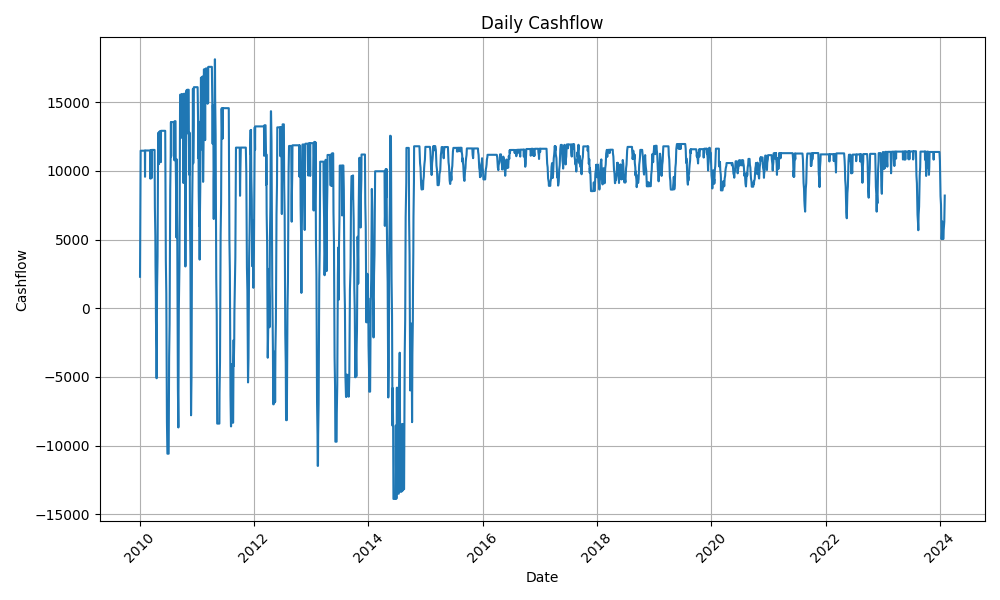
\includegraphics[width=1\textwidth]{ADX_with_short.png}
  \caption{ADX strategy Cashflow graph with short selling}
\end{figure}

\begin{figure}[H]
  \centering
  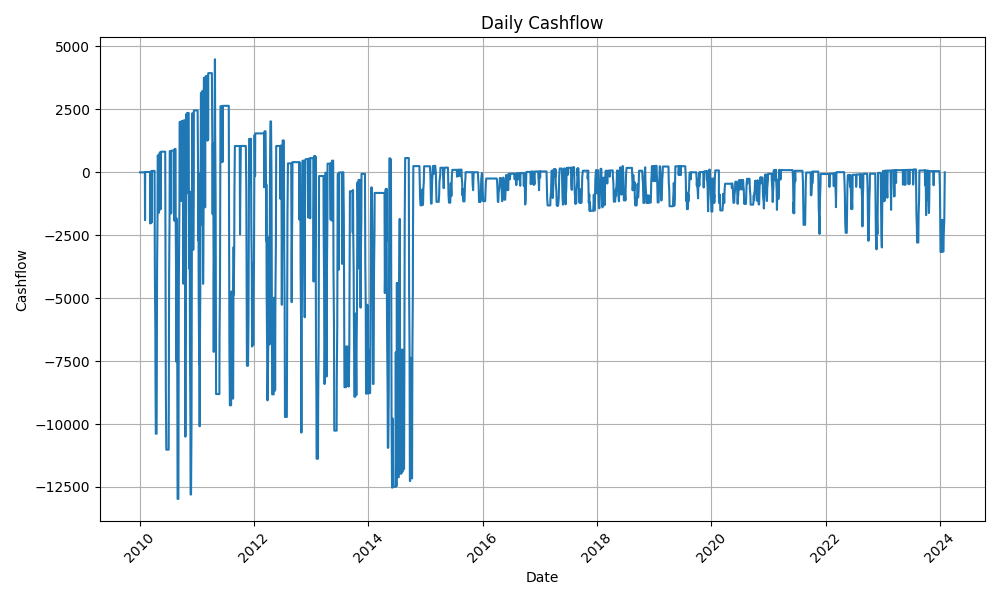
\includegraphics[width=1\textwidth]{ADX_without_short.png}
  \caption{ADX strategy Cashflow graph without short selling}
\end{figure}

\subsection{Linear Regression:-}
\begin{itemize}
    \item Linear Regression is utilized in this trading strategy to predict stock prices based on historical data. Parameters such as the previous day's close, open, VWAP, low, high, and the number of trades are used to predict the current day's close price. 
    \item If the predicted price differs from the actual price by a specified percentage, buy or sell signals are generated accordingly, with the expectation that the actual price will move towards the predicted price.
    \item We only used the normal form equation of linear regression to get the required coefficients.
    \item This algorithm is more applicable to the market as it can consider multiple factors at the same time.
    \item It can sometimes give incorrect results due to linear assumption, which is not true if the market has very high fluctuations.
\end{itemize}

\subsection{Best of All:-}
\begin{itemize}
    \item In this, we ran all the algorithms in parallel to get the best possible pnl for the given data. To achieve this, we need the C++ library OpenMP to get parallel sections in the code.
    \item For most of the cases, RSI algorithm gave the best pnl out of all the algorithms discussed above.
\end{itemize}

\subsection{Mean Reverting Pairs Trading Strategy:-}
\begin{itemize}
    \item In the Pairs Trading Strategy, the focus is on the price spread between two stocks rather than their individual prices.
    \item The algorithm calculates the spread's rolling mean and standard deviation over a specified period and generates buy or sell signals based on the spread's deviation from its mean. Buying occurs when the spread is below a negative threshold, indicating undervaluation, while selling occurs when the spread is above a positive threshold, indicating overvaluation. This strategy aims to profit from the mean-reverting behavior of the spread between the paired stocks.
    \item This type of pair trading is usually market-neutral, thus the algorithm focuses on the relative performance of the two stocks.
\end{itemize}

\subsection{Stop - Loss in Pairs Trading Strategy:-}
\begin{itemize}
    \item In the Stop-Loss in Pairs Trading Strategy, a loss-based constraint is introduced to mitigate unwanted positions. When initiating positions based on the z-score crossing a threshold, the expectation is for the z-score to revert to the mean. 
    \item However, if the z-score moves unexpectedly in the opposite direction, positions are closed when the z-score crosses a specified stop-loss threshold. This strategy aims to limit losses and protect against adverse price movements.
    \item Stop-loss orders help manage risk by automatically closing positions when losses exceed a predetermined threshold, preventing further losses.
    \item It may not give good results for highly fluctuating markets.
    \item This code is divided into two parts, one with the buy/sell given by strategy and the other by stop\_loss\_threshold. We have made an array which stores all the currently acquired positions.
    \item First we store the current position at the start of day i.e. before doing any transaction on that day.
    \item Now we update the position by going through the strategy, till here we have not added any transaction to cashflow or order stats file.
    \item then we store the sign of the current position in another variable sign.
    \item After that we check if any previous hold position crosses the threshold mark, if it crosses then we remove it from the array.
    \item Now the new current position is the size of the modified array and the sign which we have calculated previously
    \item The current day transaction is equal to final current position of the day and the position before any transaction on that day.
    \item Then if the current transaction is positive, that means we have bought the position so we update the daily\_cashflow and order\_stats accordingly. Similarly for -ve transaction.
    
\end{itemize}

\end{document}
